\documentclass[10pt,a4paper]{article}
\usepackage{tocloft}
\usepackage{commons/course}
\usepackage{booktabs}
\usepackage{graphicx}
\usepackage{tikz}
\usetikzlibrary{arrows.meta,positioning,calc,decorations.pathreplacing,fit}

\definecolor{keywordstyle}{rgb}{0.0, 0.4, 0.8}
\definecolor{stringstyle}{rgb}{0.9, 0.17, 0.31}
\definecolor{commentstyle}{rgb}{0.1, 0.6, 0.2}
\definecolor{numberstyle}{rgb}{0.4, 0.4, 0.4}
\definecolor{backgroundcolor}{rgb}{0.94, 0.97, 1.0}

\lstdefinelanguage{ShellLike}{
	morekeywords={PASS,FAIL,Passed,Failed,Running,Loading,summary,iverilog},
	sensitive=false,
	morecomment=[l]{\#},
	morestring=[b]",
}

\lstset{
	language=ShellLike,
	basicstyle=\ttfamily\scriptsize,
	keywordstyle=\color{keywordstyle}\bfseries,
	stringstyle=\color{stringstyle},
	commentstyle=\color{commentstyle},
	numbers=none,
	keepspaces=true,
	tabsize=2,
	showspaces=false,
	showstringspaces=false,
	showtabs=false,
	breaklines=true,
	breakatwhitespace=false,
	frame=single,
	backgroundcolor=\color{backgroundcolor},
}

\lstdefinestyle{verilog}{
	language=Verilog,
	basicstyle=\ttfamily\scriptsize,
	keywordstyle=\color{keywordstyle}\bfseries,
	commentstyle=\color{commentstyle},
	stringstyle=\color{stringstyle},
	numbers=left,
	numberstyle=\tiny\color{numberstyle},
	frame=single,
	backgroundcolor=\color{backgroundcolor},
	breaklines=true,
	tabsize=2,
}

\newlistof{listofproblems}{lop}{\normalsize فهرست مسائل}
\newcommand{\addproblem}[1]{\addcontentsline{lop}{listofproblems}{\protect\numberline{}#1}}


\begin{document}

\سربرگ{آزمایش هشتم}{\lr{ALU} اعداد مختلط}{}{استاد: دکتر انصاری}

\subsubsection*{خلاصه}

این آزمایش سه بخش دارد: پیمانه‌ی جمع و تفریق اعداد مختلط، پیمانه‌ی ضرب اعداد مختلط، و یک واحد پایپ‌لاین که دستورات را از یک حافظه‌ی ۳۲ کلمه‌ای می‌خواند و عملیات مختلط را روی آن‌ها انجام می‌دهد.

قید کوتاهی در انتهای صورت آزمایش آمده که در عمل تمام معماری را تعیین می‌کند:

\begin{center}
\emph{«در این آزمایش، نبایستی از واحدهای جمع کننده یا ضرب کننده بیش از یک بار استفاده شود.»}
\end{center}

یعنی در کل ماشین {یک} جمع‌کننده و {یک} ضرب‌کننده وجود دارد. تمام تصمیم‌هایی که در ادامه می‌آید — یکی بودن ماژول جمع/تفریق و ضرب، زمان‌بندی چهارمرحله‌ای ضرب، و اینکه مرحله‌ی اجرای پایپ‌لاین چند کلاکی است — پیامد مستقیم همین یک جمله است.

\subsubsection*{نمایش عدد مختلط}

هر عدد مختلط یک زوج از دو مؤلفه‌ی {علامت‌دار مکمل ۲} هشت‌بیتی است که در یک کلمه‌ی ۱۶ بیتی بسته‌بندی می‌شود:

\begin{center}
\lr{word = \{ imag[7:0], real[7:0] \}} \qquad بازه‌ی هر مؤلفه: $-128$ تا $+127$
\end{center}

نتایج {اشباع} می‌شوند نه سرریز: مؤلفه‌ای که از بازه بیرون بزند به $-128$ یا $+127$ چسبانده می‌شود و پرچمی بالا می‌رود. برای ماشینی که کارش حساب روی کمیت‌های اندازه‌گیری‌شده است این رفتار مفیدتر است — مقداری که خیلی بزرگ شده باید «خیلی بزرگ» خوانده شود، نه اینکه بی‌سروصدا علامتش عوض شود. مثلا $100 \times 100 = 10000$ با سرریز عادی به $16$ تبدیل می‌شد که هیچ ربطی به پاسخ درست ندارد.

\subsubsection*{چرا جمع/تفریق و ضرب یک ماژول‌اند}

ضرب دو عدد مختلط به {چهار} ضرب حقیقی و {دو} جمع حقیقی نیاز دارد:

\[
(a_r + j\,a_i)(b_r + j\,b_i) \;=\; (a_r b_r - a_i b_i) \;+\; j\,(a_r b_i + a_i b_r)
\]

و جمع دو عدد مختلط به دو جمع حقیقی دیگر. اگر بخش الف و بخش ب دو ماژول جدا می‌بودند، سطح بالای ماشین {دو} جمع‌کننده می‌داشت — دقیقا همان چیزی که قید بالا ممنوع کرده است.

بنابراین هر دو عملیات در یک ماژول به نام \lr{complex\_alu} زندگی می‌کنند که داخل آن دقیقا یک \lr{mul\_unit} و یک \lr{add\_unit} قرار دارد. بخش الف و بخش ب دو {حالت کاری} این ماژول‌اند و هر کدام تست‌بنچ مستقل خودشان را دارند. بهایی که برای این قید پرداخت می‌شود در {زمان} است نه در سطح: ماژول به‌جای ترکیبی، ترتیبی است.

\subsubsection*{زمان‌بندی واحد مشترک}

\begin{center}
\begin{latin}
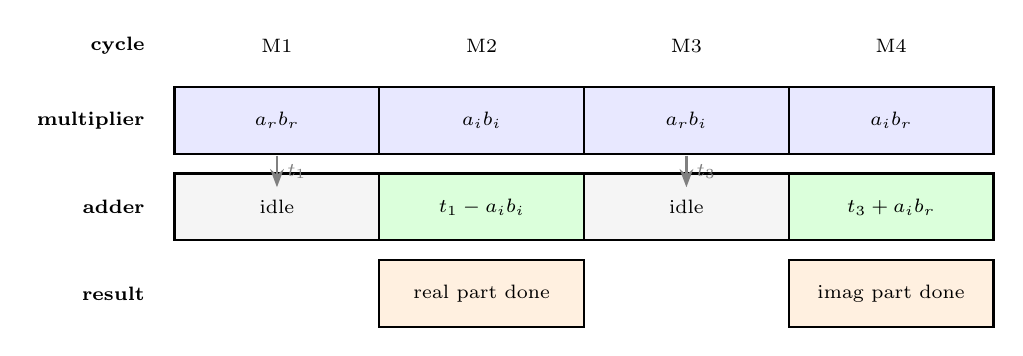
\begin{tikzpicture}[
  cyc/.style={draw, minimum height=0.85cm, minimum width=2.6cm, align=center,
              font=\scriptsize, inner sep=1pt},
  lbl/.style={font=\scriptsize\bfseries, anchor=east},
  >=Stealth, thick
]
  \node[lbl] at (-0.25,0.95)  {cycle};
  \node[font=\scriptsize] at (1.3,0.95)  {M1};
  \node[font=\scriptsize] at (3.9,0.95)  {M2};
  \node[font=\scriptsize] at (6.5,0.95)  {M3};
  \node[font=\scriptsize] at (9.1,0.95)  {M4};

  \node[lbl] at (-0.25,0)  {multiplier};
  \node[cyc, fill=blue!9]  at (1.3,0)  {$a_r b_r$};
  \node[cyc, fill=blue!9]  at (3.9,0)  {$a_i b_i$};
  \node[cyc, fill=blue!9]  at (6.5,0)  {$a_r b_i$};
  \node[cyc, fill=blue!9]  at (9.1,0)  {$a_i b_r$};

  \node[lbl] at (-0.25,-1.1)  {adder};
  \node[cyc, fill=black!4]   at (1.3,-1.1)  {idle};
  \node[cyc, fill=green!14]  at (3.9,-1.1)  {$t_1 - a_i b_i$};
  \node[cyc, fill=black!4]   at (6.5,-1.1)  {idle};
  \node[cyc, fill=green!14]  at (9.1,-1.1)  {$t_3 + a_i b_r$};

  \node[lbl] at (-0.25,-2.2)  {result};
  \node[cyc, fill=orange!12] at (3.9,-2.2)  {real part done};
  \node[cyc, fill=orange!12] at (9.1,-2.2)  {imag part done};

  \draw[->, gray] (1.3,-0.45) -- (1.3,-0.85) node[midway,right,font=\scriptsize]{$t_1$};
  \draw[->, gray] (6.5,-0.45) -- (6.5,-0.85) node[midway,right,font=\scriptsize]{$t_3$};
\end{tikzpicture}
\end{latin}
\end{center}

نکته‌ی اصلی این زمان‌بندی در ستون‌های \lr{M2} و \lr{M4} است: جمع‌کننده روی حاصل‌ضربی کار می‌کند که {در همان کلاک} از ضرب‌کننده بیرون می‌آید، در حالی که ضرب‌کننده هم بی‌کار نمانده و مشغول حاصل‌ضرب بعدی است. بدون این هم‌پوشانی، ضرب مختلط $4$ کلاک ضرب به‌علاوه‌ی $2$ کلاک جمع، یعنی $6$ کلاک، طول می‌کشید. با آن، $4$ کلاک — و هیچ واحد اضافه‌ای هم به مدار اضافه نشده است.

\begin{center}
\begin{tabular}{@{}lll@{}}
\toprule
{عملیات} & {کلاک اشغال واحد مشترک} & {علت} \\
\midrule
\lr{ADD / SUB} & $2$ & دو جمع حقیقی، یک جمع‌کننده \\
\lr{MUL}            & $4$ & چهار ضرب حقیقی، یک ضرب‌کننده \\
\bottomrule
\end{tabular}
\end{center}

هر دو عدد در تست‌بنچ‌ها {صریحا} بررسی شده‌اند، نه فقط نتیجه‌ی عددی؛ چون درست بودن پاسخ به‌تنهایی نشان نمی‌دهد که مدار واقعا از یک واحد استفاده کرده باشد.

\begin{latin}
\lstinputlisting[style=verilog]{../rtl/complex_alu.v}
\end{latin}

دو واحد مشترک خودشان کوچک‌اند. توجه کنید که تفریق واحد دومی نیست: \lr{x - y} همان جمع‌کننده با معکوس کردن \lr{y} و یک رقم نقلی ورودی است، که دقیقا همان چیزی است که سنتزکننده می‌سازد.

\begin{latin}
\lstinputlisting[style=verilog]{../rtl/mul_unit.v}
\lstinputlisting[style=verilog]{../rtl/add_unit.v}
\end{latin}

پهنای جمع‌کننده $17$ بیت است، چون همین یک واحد باید دو کار خیلی متفاوت را انجام دهد: جمع دو مؤلفه‌ی $8$ بیتی (که $9$ بیت کافی بود) و ترکیب دو حاصل‌ضرب جزئی $16$ بیتی (که $17$ بیت لازم دارد).

\subsubsection*{ماشین: مجموعه دستورات و حافظه}

صورت آزمایش می‌گوید ماشین یک حافظه‌ی $32$ کلمه‌ای دارد و واحد پایپ‌لاین دستورات را از همان حافظه می‌خواند. هر کلمه $32$ بیت است:

\begin{center}
\begin{latin}
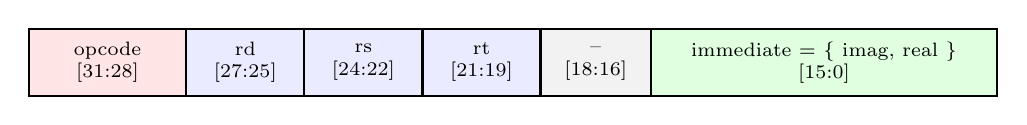
\begin{tikzpicture}[
  f/.style={draw, minimum height=0.85cm, align=center, font=\scriptsize, inner sep=2pt},
  >=Stealth, thick
]
  \node[f, minimum width=2.0cm, fill=red!10]    (op) at (0,0)     {opcode\\\lr{[31:28]}};
  \node[f, minimum width=1.5cm, fill=blue!8]    (rd) at (1.75,0)  {rd\\\lr{[27:25]}};
  \node[f, minimum width=1.5cm, fill=blue!8]    (rs) at (3.25,0)  {rs\\\lr{[24:22]}};
  \node[f, minimum width=1.5cm, fill=blue!8]    (rt) at (4.75,0)  {rt\\\lr{[21:19]}};
  \node[f, minimum width=1.4cm, fill=black!5]   (un) at (6.2,0)   {--\\\lr{[18:16]}};
  \node[f, minimum width=4.4cm, fill=green!12]  (im) at (9.1,0)   {immediate = \{ imag, real \}\\\lr{[15:0]}};
\end{tikzpicture}
\end{latin}
\end{center}

\begin{center}
\begin{tabular}{@{}lll p{5.6cm}@{}}
\toprule
{کد} & {دستور} & {اثر} & {توضیح} \\
\midrule
\lr{0} & \lr{NOP}  & --                     & حباب پایپ‌لاین \\
\lr{1} & \lr{LDI}  & \lr{rd $\leftarrow$ imm}      & تنها راه وارد کردن ثابت \\
\lr{2} & \lr{MOV}  & \lr{rd $\leftarrow$ rs}       & بدون استفاده از \lr{ALU} \\
\lr{3} & \lr{ADD}  & \lr{rd $\leftarrow$ rs + rt}  & دو کلاک جمع‌کننده \\
\lr{4} & \lr{SUB}  & \lr{rd $\leftarrow$ rs - rt}  & دو کلاک جمع‌کننده \\
\lr{5} & \lr{MUL}  & \lr{rd $\leftarrow$ rs $\times$ rt} & چهار کلاک ضرب‌کننده \\
\lr{F} & \lr{HALT} & --                     & واکشی را متوقف می‌کند \\
\bottomrule
\end{tabular}
\end{center}

ثبات‌ها هشت‌تا و هرکدام یک عدد مختلط کامل‌اند. \lr{LDI} و \lr{MOV} عمدا از \lr{ALU} استفاده نمی‌کنند؛ این باعث می‌شود در بخش تست بشود {اثر خالص پایپ‌لاین} را از {اثر واحد مشترک} جدا اندازه گرفت.

\subsubsection*{پایپ‌لاین}

\begin{center}
\begin{latin}
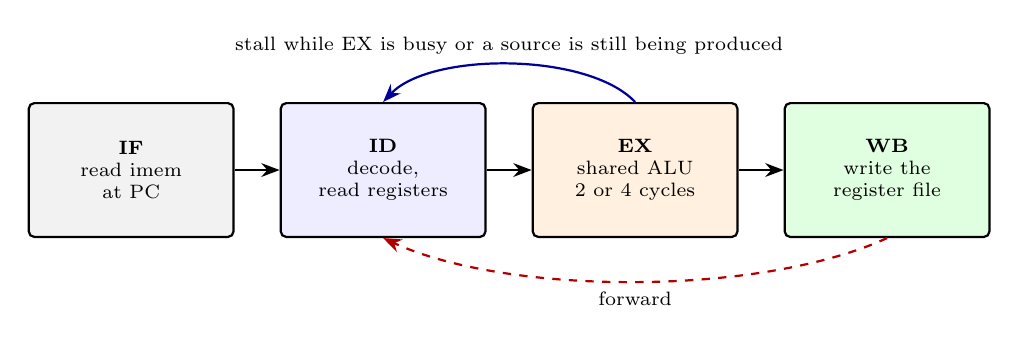
\begin{tikzpicture}[
  stg/.style={draw, rounded corners=2pt, minimum height=1.7cm, minimum width=2.6cm,
              align=center, font=\scriptsize},
  >=Stealth, thick
]
  \node[stg, fill=black!5]   (if) at (0,0)    {\textbf{IF}\\read imem\\at PC};
  \node[stg, fill=blue!7]    (id) at (3.2,0)  {\textbf{ID}\\decode,\\read registers};
  \node[stg, fill=orange!12] (ex) at (6.4,0)  {\textbf{EX}\\shared ALU\\2 or 4 cycles};
  \node[stg, fill=green!12]  (wb) at (9.6,0)  {\textbf{WB}\\write the\\register file};

  \draw[->] (if) -- (id);
  \draw[->] (id) -- (ex);
  \draw[->] (ex) -- (wb);

  \draw[->, red!70!black, dashed] (wb.south) ++(0,0) .. controls (8.0,-1.6) and (4.8,-1.6) ..
      (id.south) node[midway, below, font=\scriptsize, black]{forward};

  \draw[<-, blue!60!black] (id.north) ++(0,0) .. controls (3.8,1.5) and (5.8,1.5) ..
      (ex.north) node[midway, above, font=\scriptsize, black]{stall while EX is busy or a source is still being produced};
\end{tikzpicture}
\end{latin}
\end{center}

پیامد جالب قید تک‌واحدی این است که مرحله‌ی \lr{EX} خودش {نمی‌تواند} پایپ‌لاین شود: وقتی فقط یک ضرب‌کننده وجود دارد، تنها یک حاصل‌ضرب می‌تواند در جریان باشد. اما \lr{IF} و \lr{ID} و \lr{WB} همچنان با \lr{EX} هم‌پوشانی دارند — در حالی که یک ضرب چهار کلاک طول می‌کشد، دستور بعدی واکشی و کدگشایی شده و نتیجه‌ی دستور قبلی در حال نوشته شدن است. به بیان دیگر \lr{EX} گلوگاه گذردهی است، ولی این یک {انتخاب اعلام‌شده} است نه یک اشتباه.

دو قفل داخلی درستی را تضمین می‌کنند:

\textbf{الف) قفل منبع.} مرحله‌ی \lr{EX} فقط وقتی دستور تازه می‌پذیرد که آزاد باشد (یا در همین کلاک آزاد شود). بنابراین یک عملیات طولانی، کدگشایی و واکشی را پشت خودش متوقف می‌کند.

\textbf{ب) قفل داده و ارسال به جلو.} دستوری که ثبات مبدأش هنوز در \lr{EX} در حال تولید است، در \lr{ID} منتظر می‌ماند. به‌محض اینکه تولیدکننده به \lr{WB} برسد، مقدار مستقیما به مرحله‌ی کدگشایی {ارسال به جلو} می‌شود. نتیجه این است که انتظار دقیقا به اندازه‌ای است که باید باشد و نه یک کلاک بیشتر — عددی که در بخش تست اندازه‌گیری شده است.

\textbf{ج) اعلام پایان کار.} سیگنال \lr{halted} فقط یک چیز می‌گوید: واکشی متوقف شده است. ولی در همان لحظه ممکن است آخرین دستور هنوز در \lr{EX} باشد، یا نتیجه‌اش در ثبات \lr{WB} منتظر لبه‌ی بعدی کلاک نشسته باشد. هر کسی که با دیدن \lr{halted} فایل ثبات را بخواند، مقدار قدیمی می‌بیند.

به همین دلیل خروجی جداگانه‌ای به نام \lr{finished} وجود دارد که علاوه بر توقف واکشی، {خالی بودن پایپ‌لاین} را هم شرط می‌کند:

\begin{latin}
\begin{lstlisting}[style=verilog,numbers=none]
assign finished = halted && !ex_v && !wb_v;
\end{lstlisting}
\end{latin}

این تمایز در نگاه اول بی‌اهمیت به نظر می‌رسد ولی دقیقا همان چیزی است که در اولین نسخه‌ی تست‌بنچ باعث خطا شد: تست با دیدن \lr{halted} ثبات‌ها را می‌خواند و نتیجه‌ی آخرین دستور را از دست می‌داد. راه درست، اصلاح {واسط} بود نه اضافه کردن تاخیر به تست.

نکته‌ی ظریف دیگری که ارزش گفتن دارد: ارسال به جلو از \lr{WB} به \lr{ID} {لازم} است، نه یک بهینه‌سازی اختیاری. آرایه‌ی ثبات‌ها در لبه‌ی کلاک نوشته می‌شود و خواندن آن ترکیبی است، پس دستوری که در همان کلاکِ نوشتن، همان ثبات را می‌خواند مقدار {قدیمی} را می‌بیند. بدون این مسیر، برنامه‌های وابسته پاسخ غلط می‌دادند.

\begin{latin}
\lstinputlisting[style=verilog]{../rtl/complex_cpu.v}
\end{latin}

\subsubsection*{شکل موج}

\begin{center}
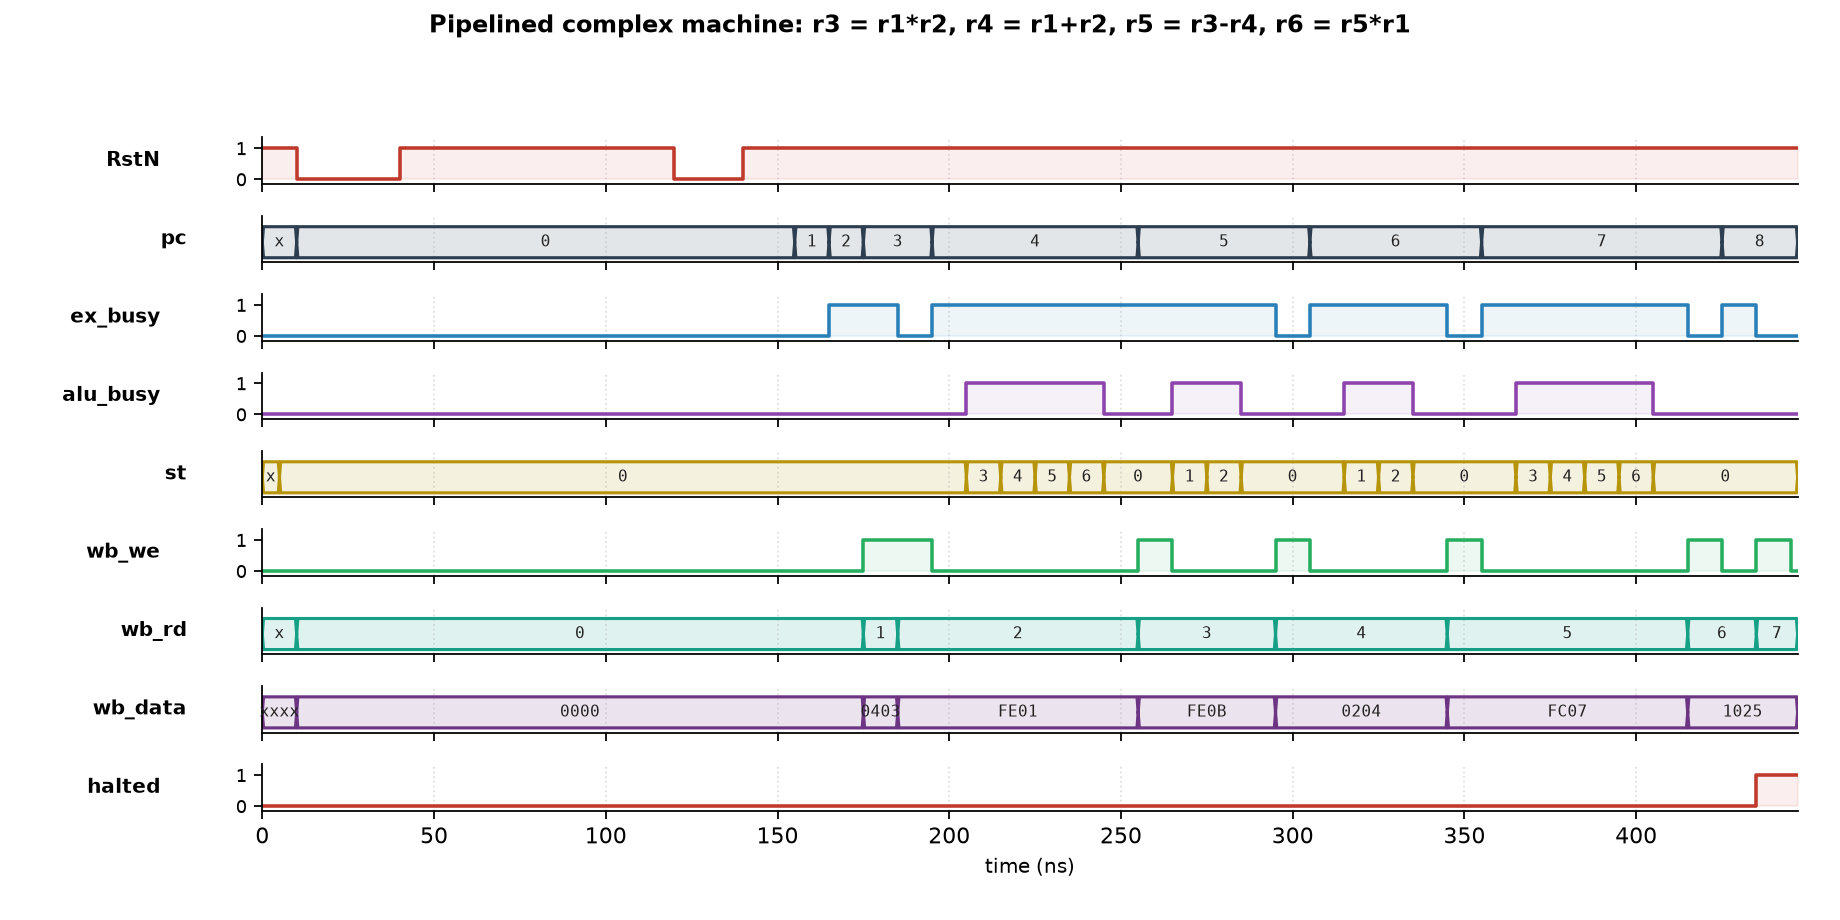
\includegraphics[width=\textwidth]{figs/wave_complex_cpu.png}\\[0.4em]
\end{center}

برنامه‌ی نمایش‌داده‌شده این است:

\begin{center}
\begin{tabular}{@{}lll@{}}
\toprule
{دستور} & {محاسبه} & {مقدار نوشته‌شده} \\
\midrule
\lr{LDI r1, 3+4j}   & --                      & \lr{0x0403} \\
\lr{LDI r2, 1-2j}   & --                      & \lr{0xFE01} \\
\lr{MUL r3, r1, r2} & $(3+4j)(1-2j) = 11-2j$  & \lr{0xFE0B} \\
\lr{ADD r4, r1, r2} & $(3+4j)+(1-2j) = 4+2j$  & \lr{0x0204} \\
\lr{SUB r5, r3, r4} & $(11-2j)-(4+2j) = 7-4j$ & \lr{0xFC07} \\
\lr{MUL r6, r5, r1} & $(7-4j)(3+4j) = 37+16j$ & \lr{0x1025} \\
\lr{MOV r7, r6}     & --                      & \lr{0x1025} \\
\bottomrule
\end{tabular}
\end{center}

سه چیز در شکل‌موج قابل دیدن است. اول، سیگنال \lr{st} که حالت داخلی \lr{ALU} است: برای هر \lr{MUL} دنباله‌ی $3,4,5,6$ (یعنی \lr{M1} تا \lr{M4}) و برای هر \lr{ADD} و \lr{SUB} دنباله‌ی $1,2$ دیده می‌شود — همان زمان‌بندی جدول بالا. دوم، \lr{alu\_busy} هرگز دو عملیات را هم‌زمان نشان نمی‌دهد، که همان قید تک‌واحدی است. سوم، \lr{pc} در حالی جلو می‌رود که \lr{ALU} هنوز مشغول است: این خودِ هم‌پوشانی پایپ‌لاین است.

توجه کنید که دو نوشتن آخر (\lr{r6} و \lr{r7}) پشت سر هم و بدون فاصله انجام می‌شوند، چون \lr{MOV} از \lr{ALU} استفاده نمی‌کند و بلافاصله پس از آزاد شدن \lr{EX} وارد آن می‌شود.

\subsubsection*{تست‌ها}

پنج تست وجود دارد که اولین آن‌ها اصلا شبیه‌سازی نیست.

\textbf{۱) بررسی منبع.} قید «بیش از یک بار استفاده نشود» یک ویژگی {متن مدار} است، نه یک ویژگی شکل‌موج. هیچ شبیه‌سازی‌ای نمی‌تواند نشان دهد که دو ضرب‌کننده در مدار وجود ندارد — مداری با دو ضرب‌کننده همان جواب‌های درست را می‌دهد. بنابراین اسکریپت تست پیش از هر شبیه‌سازی، تعداد نمونه‌سازی‌های \lr{mul\_unit}، \lr{add\_unit} و \lr{complex\_alu} را در کل \lr{RTL} می‌شمارد و اگر هرکدام بیش از یکی باشد تست را رد می‌کند.

\textbf{۲ و ۳) بخش الف و بخش ب.} هر کدام یک مدل مرجع دارند که با حساب صحیح ساده نوشته شده — بدون ماشین حالت و بدون زمان‌بندی — و بنابراین هیچ اشتباهی را با طراحی شریک نمی‌شود. پوشش شامل تمام ترکیب‌های نه مقدار مرزی روی هر چهار مؤلفه (یعنی $9^4 = 6561$ حالت برای هر عملیات) به‌علاوه‌ی یک جاروب تصادفی است. علاوه بر مقدار عددی، پرچم اشباع و {تعداد کلاک} هر عملیات هم بررسی می‌شود.

\begin{latin}
\lstinputlisting[style=verilog]{../tb/tb_complex_addsub.v}
\end{latin}

\begin{latin}
\lstinputlisting[style=verilog]{../tb/tb_complex_mul.v}
\end{latin}

\textbf{۴) ماشین در برابر مدل مرجع.} مدل یک مفسر ساده‌ی همان برنامه است: بدون پایپ‌لاین، بدون توقف و بدون واحد مشترک. توافق با آن یعنی قفل‌ها و مسیر ارسال به جلو دقیقا همان نتیجه‌ای را می‌سازند که اجرای دستورات یکی‌یکی می‌ساخت.

بیشتر کار را {برنامه‌های تصادفی} انجام می‌دهند. برنامه‌ی دست‌نویس فقط الگوهای وابستگی‌ای را پوشش می‌دهد که نویسنده‌اش به آن‌ها فکر کرده؛ صد و پنجاه برنامه‌ی تصادفی زنجیره‌های وابستگی، استفاده‌ی مجدد از ثبات‌ها و هم‌نامی عملوندها را پوشش می‌دهند که هیچ‌کس آن‌ها را عمدا نمی‌نویسد.

\begin{latin}
\lstinputlisting[style=verilog]{../tb/tb_complex_cpu.v}
\end{latin}

\textbf{۵) ادعاهای ساختاری پایپ‌لاین.} مقایسه با مدل مرجع نشان می‌دهد ماشین عدد {درست} را می‌دهد، ولی درباره‌ی اینکه {چرا} این‌قدر طول می‌کشد چیزی نمی‌گوید — ماشینی که بی‌سروصدا هر دستور را جداگانه و بدون هم‌پوشانی اجرا کند هم همان تست را پاس می‌کند. تست پنجم دقیقا همین را اندازه می‌گیرد:

\begin{center}
\begin{tabular}{@{}l r p{6.0cm}@{}}
\toprule
{سناریو} & {کلاک} & {نتیجه‌گیری} \\
\midrule
۱۶ دستور تک‌کلاکی مستقل    & $19$  & حدود یک کلاک برای هر دستور؛ بدون هم‌پوشانی دست‌کم $3\times16$ لازم بود \\
۱۶ ضرب مستقل               & $102$ & گلوگاه، ضرب‌کننده‌ی مشترک است نه پایپ‌لاین \\
۱۶ ضرب زنجیره‌ای وابسته     & $117$ & هزینه‌ی قفل داده \\
\bottomrule
\end{tabular}
\end{center}

سطر آخر عدد قشنگی می‌دهد: اختلاف $117 - 102 = 15$ کلاک است و تعداد جفت‌های وابسته هم دقیقا $15$ تاست. یعنی قفل داده {دقیقا یک کلاک} برای هر وابستگی هزینه دارد — همان یک کلاکی که مصرف‌کننده منتظر می‌ماند تا تولیدکننده از \lr{EX} به \lr{WB} برود و مسیر ارسال به جلو در دسترس شود. این تساوی در تست‌بنچ به‌صورت یک شرط دقیق نوشته شده، نه به‌صورت یک بازه.

\begin{latin}
\lstinputlisting[style=verilog]{../tb/tb_complex_cpu_spec.v}
\end{latin}

\subsubsection*{نتایج تست}

\begin{latin}
\lstinputlisting[basicstyle=\ttfamily\scriptsize]{figs/test_run_output.txt}
\end{latin}

\subsubsection*{جمع‌بندی}

درس اصلی این آزمایش این است که یک قید منابع، معماری را عوض می‌کند نه فقط اندازه‌اش را. با اجازه‌ی داشتن چهار ضرب‌کننده، ضرب مختلط یک مدار ترکیبی یک‌کلاکی می‌شد و مرحله‌ی اجرا هم مثل بقیه‌ی مراحل پایپ‌لاین می‌شد. با یک ضرب‌کننده، همان عملیات به یک ماشین حالت چهارکلاکی تبدیل می‌شود و در نتیجه پایپ‌لاین به قفل و توقف نیاز پیدا می‌کند — چیزی که بدون آن قید اصلا لازم نبود.

نکته‌ی دوم درباره‌ی تست است. چهار تست‌بنچ این آزمایش هیچ‌کدام نمی‌توانند نشان دهند که قید اصلی رعایت شده است، چون مداری با دو ضرب‌کننده همان جواب‌های درست را در زمان کمتری می‌دهد و همه‌ی آن‌ها را پاس می‌کند. برای ویژگی‌هایی که درباره‌ی {ساختار} مدارند و نه رفتار آن، باید سراغ خود متن رفت؛ به همین دلیل شمارش نمونه‌سازی‌ها به‌عنوان اولین تست به اسکریپت اضافه شد.

\pagebreak
\subsubsection*{خروجی سنتز (\lr{Quartus Prime})}

طرح روی \lr{Intel Quartus Prime Lite Edition 21.1.0} با موجودیت سطح‌بالای \lr{complex\_cpu} سنتز و Place \& Route شد. دستگاه هدف: \lr{Cyclone V} (\lr{5CGXFC7C7F23C8}).

\begin{center}
\begin{tabular}{@{}lr@{}}
\toprule
{مورد} & {نتیجه} \\
\midrule
وضعیت کامپایل & موفق ($0$ خطا، $19$ هشدار) \\
\lr{Logic utilization (ALMs)} & $699 / 56480$ ($1\%$) \\
\lr{Total registers} & $1272$ \\
\lr{Total pins} & $90 / 268$ ($34\%$) \\
\lr{Block memory bits} & $0$ \\
\lr{DSP Blocks} & $1 / 156$ ($<1\%$) \\
\bottomrule
\end{tabular}
\end{center}

\begin{center}

\includegraphics[width=\textwidth]{figs/quartus_synthesis.jpg}
\end{center}

\end{document}
